\def\documentauthor{Carlos Salinas}
\def\documenttitle{MA 166: Quiz {\hwnum} Solutions}
\def\hwnum{4}
\def\shorttitle{MA 166 HW {\hwnum} Sols}
\def\coursename{MA166}
\def\documentsubject{calculus ii}
\def\authoremail{salinac@purdue.edu}

\documentclass[12pt]{article}
\usepackage{geometry}
\usepackage[dvipsnames]{xcolor}
\usepackage[
    breaklinks,
    bookmarks=true,
    % colorlinks=true,
    pageanchor=false,
    linkcolor=black,
    anchorcolor=black,
    citecolor=black,
    filecolor=black,
    menucolor=black,
    runcolor=black,
    urlcolor=black,
    hyperindex=false,
    hyperfootnotes=true,
    pdftitle={\shorttitle},
    pdfauthor={\documentauthor},
    pdfkeywords={\documentsubject},
    pdfsubject={\coursename}
    ]{hyperref}

% Use symbols instead of numbers
\renewcommand*{\thefootnote}{\fnsymbol{footnote}}

%% Math
\usepackage{amsmath}
\usepackage{amsthm}
\usepackage{amssymb}
\usepackage{mathtools}

%%PDFTeX specific
\usepackage[mathcal]{euscript}
\usepackage{mathrsfs}
\usepackage{dsfont}
\usepackage{wasysym}

\usepackage[LAE,LFE,T2A,T1]{fontenc}
\usepackage[utf8]{inputenc}
\usepackage[farsi,french,german,spanish,russian,english]{babel}
\babeltags{pa=farsi,
           fr=french,
           de=german,
           es=spanish,
           ru=russian,
           en=english}
\def\spanishoptions{mexico}

\selectlanguage{english}

\newcommand{\textfa}[1]{\beginR\textpa{#1}\endR}

\usepackage{cmap}
\usepackage{CJKutf8}
\newcommand{\textkr}[1]{\begin{CJK}{UTF8}{mj}#1\end{CJK}}
\newcommand{\textjp}[1]{\begin{CJK}{UTF8}{min}#1\end{CJK}}
\newcommand{\textzh}[1]{\begin{CJK}{UTF8}{bsmi}#1\end{CJK}}

%% Misc
\usepackage{graphicx}
\usepackage{cutwin}
\graphicspath{{figures/}}

\usepackage{microtype}
\usepackage{multicol}
\usepackage[inline]{enumitem}
\usepackage{listings}
\usepackage{mleftright}
\mleftright

%% Theorems and definitions
\theoremstyle{plain}
\newtheorem{theorem}{Theorem}
\newtheorem{proposition}[theorem]{Proposition}
\newtheorem{corollary}[theorem]{Corollary}
\newtheorem{claim}[theorem]{Claim}
\newtheorem{lemma}[theorem]{Lemma}
\newtheorem{axiom}[theorem]{Axiom}

\newtheorem*{corollary*}{Corollary}
\newtheorem*{claim*}{Claim}
\newtheorem*{lemma*}{Lemma}
\newtheorem*{proposition*}{Proposition}
\newtheorem*{theorem*}{Theorem}

\theoremstyle{definition}
\newtheorem{definition}{Definition}
\newtheorem{example}{Examples}
\newtheorem{examples}[example]{Examples}
\newtheorem{exercise}{Exercise}
\newtheorem{problem}[exercise]{Problem}

\newtheorem*{definition*}{Definition}
\newtheorem*{example*}{Examples}
\newtheorem*{examples*}{Examples}
\newtheorem*{exercise*}{Exercise}
\newtheorem*{problem*}{Problem}

\theoremstyle{remark}
\newtheorem{remark}{Remark}
\newtheorem{remarks}[remark]{Remarks}
\newtheorem{observation}[remark]{Observation}
\newtheorem{observations}[remark]{Observations}

\newtheorem*{remark*}{**Remark**}
\newtheorem*{remarks*}{**Remarks**}
\newtheorem*{observation*}{**Observation**}
\newtheorem*{observations*}{**Observations**}

%% Commands and operators
%% Redefinitions & commands
\newcommand{\nsubset}{\ensuremath{\not\subset}}
\newcommand{\nsupset}{\ensuremath{\not\supset}}
\newcommand\minus{\ensuremath{\null\smallsetminus}}
\renewcommand\qedsymbol{\ensuremath{\null\hfill\blacksquare}}

%% Commands and operators
\DeclareMathOperator{\id}{id}
\DeclareMathOperator{\im}{im}

%% Linear algebra
\DeclareMathOperator{\proj}{proj}
\DeclareMathOperator{\comp}{comp}

%% Differential operators
\DeclareMathOperator{\Curl}{curl}
\DeclareMathOperator{\Div}{div}
\DeclareMathOperator{\Grad}{grad}
\DeclareMathOperator{\Lap}{\Delta}
\DeclareMathOperator{\diff}{d\!}

%% Misc
\newcommand{\bbC}{\mathbb{C}}
\newcommand{\bbCP}{\mathbb{CP}}
\newcommand{\bbH}{\mathbb{H}}
\newcommand{\bbN}{\mathbb{N}}
\newcommand{\bbQ}{\mathbb{Q}}
\newcommand{\bbR}{\mathbb{R}}
\newcommand{\bbRP}{\mathbb{RP}}
\newcommand{\bbZ}{\mathbb{Z}}

\newcommand{\bfC}{\mathbf{C}}
\newcommand{\bfCP}{\mathbf{CP}}
\newcommand{\bfH}{\mathbf{H}}
\newcommand{\bfN}{\mathbf{N}}
\newcommand{\bfQ}{\mathbf{Q}}
\newcommand{\bfR}{\mathbf{R}}
\newcommand{\bfRP}{\mathbf{RP}}
\newcommand{\bfZ}{\mathbf{Z}}

\newcommand{\calA}{\mathcal{A}}
\newcommand{\calB}{\mathcal{B}}
\newcommand{\calC}{\mathcal{C}}
\newcommand{\calS}{\mathcal{S}}
\newcommand{\calT}{\mathcal{T}}
\newcommand{\calU}{\mathcal{U}}
\newcommand{\calV}{\mathcal{V}}

\newcommand{\scrL}{\mathscr{L}}
\newcommand{\scrO}{\mathscr{O}}
\newcommand{\scrS}{\mathscr{S}}

\newcommand{\bfa}{\mathbf{a}}
\newcommand{\bfb}{\mathbf{b}}
\newcommand{\bfc}{\mathbf{c}}
\newcommand{\bfu}{\mathbf{u}}
\newcommand{\bfv}{\mathbf{v}}
\newcommand{\bfw}{\mathbf{w}}

\begin{document}
\author{TA: \href{mailto:\authoremail}{\documentauthor}}
\title{\documenttitle}
\date{\today}
\maketitle

You have \textbf{15 minutes} to complete this quiz. You may work in groups,
but you are not allowed to use any other resources.
\\\\
%% Quiz problems
% \begin{problem}[Easy]
% Shown is the graph of a force function (in Newtons) that increases to its
% maximum value and then remains constant. How much work $W$ is done by the
% force in moving an object a distance of $24$ meters?
% \begin{center}
% 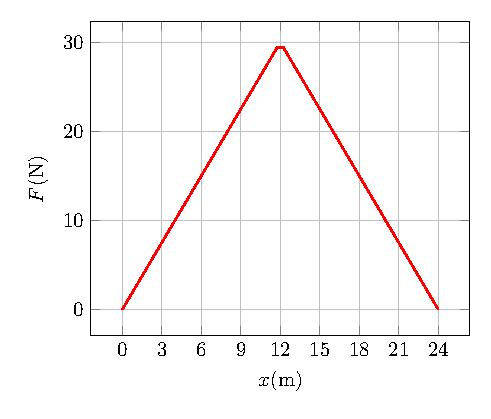
\includegraphics[scale=0.75]{../figures/quiz-4-fig-1}
% \end{center}
% \end{problem}
\begin{problem}[Medium]
\begin{enumerate}[label=(\alph*)]
\item Find the volume $V$ of the solid obtained by rotating the region
  enclosed by the curves $y=x^2$ and $y=x^3$ about the $x$-axis.
\item The region inside the circle $x^2+y^2=1$ and to the right of the line
  $x=1/2$ is rotated about the $y$-axis. Use the method of shells to find
  the volume of the resulting solid.
\item Find the indefinite integral
\[
\int x^5e^{-x}\diff x.
\]
\end{enumerate}
\end{problem}
\begin{problem}
  The tank pictured below is full of water. Let $a=6$, $b=4$, and $c=8$. Do
  not worry about the spout. Set up the integral which gives the work
  required to pump all of the water over the top. Do not evaluate the
  integral. (Water weighs $62.5$ lbs/ft$^3$, accounting for gravity).
\begin{center}
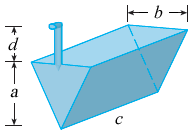
\includegraphics[scale=0.5]{../figures/hw-7-fig-2}
\end{center}
\end{problem}
\begin{problem}
A solid $S$ has a square base on the $xy$-plane with four points $(1,0)$,
$(0,1)$, $(-1,0)$ and $(0,-1)$ as vertices. Its cross-section perpendicular
to the $x$-axis are equilateral triangles. Find an expression for the
volume of $S$.
\end{problem}
\newpage
\section*{Solutions}
\begin{proof}[Solution to Problem 1]
(a) First, we need to find where $y=x^2$ and $y=x^3$ intersect. We set the
equations equal to each other and solve for $x$
\begin{align*}
x^3&=x^2\\
x^3-x^2&=0\\
x^2(x-1)&=0
\end{align*}
so $x=0$ or $x=1$. Next, since we are trying to solve for the volume using
the washer method, we need to find an expression for the cross-sectional
area preferably in terms of $x$. Now, to make sure we are not off by a
sign, we need to find out which of the curves achieves greater values from
$0\leq x\leq 1$, i.e., which curve is above the other. First, we note that
for any $0\leq x\leq 1$, the following inequality holds
\[
x\leq 1,
\]
right? Then multiplying both sides by $x^2$, we have
\[
x^3\leq x^2.
\footnote{This exactly ties in with your intuition that cubes of fractions are
smaller than squares of fractions, this is always true for powers of
numbers between $0$ and $1$ (not including $0$ or $1$). For example
$(1/2)^2=1/4$ but $(1/2)^3=1/8$. If you want a quick way to tell which
fraction is greater use the following method: Let $a$, $b$, $c$ and $d$ be
integers with $c$ and $d$ not equal to $0$ (so we can divide by them), then
$a/b<c/d$ if and only if $ad<bc$.}
\]
This tells us that $y=x^3$ will be under $y=x^2$ on the interval $0\leq
x\leq 1$. Now we are ready to find the cross-sectional area. Let me be more
systematic so you can understand where all of this is coming from, but when
it comes to the exam, feel free to leave off any step since what really
matters is that you get the correct answer. Back to the problem. Let us
label $y_1=x^2$ and $y_2=x^3$. Then the circular cross-sectional area made
by the $y_1$ is $A_1(y_1)=\pi {y_1}^2$ and the one made by
$A_2(y_2)=\pi{y_2}^2$. We can rewrite these in terms of $x$ like so
\begin{align*}
A_1(x)&=\pi \left(x^2\right)^2=\pi x^4\\
A_2(x)&=\pi \left(x^3\right)^2=\pi x^6.
\end{align*}
What we are really after is the area between these two circular
cross-section, so we take their difference
\[
A(x)=A_1(x)-A_2(x)=\pi x^4-\pi x^6=\pi\left(x^4-x^6\right).
\]
So far so good? Now, all we need to do is integrate this with respect to
$x$ as we move from $0$ to $1$, and we have
\begin{align*}
\int_0^1 A(x)\diff x
&=\int_0^1 \pi\left(x^4-x^6\right)\diff x\\
&=\pi\int_0^1 x^4-x^6\diff x\\
&=\pi\left(\left.\tfrac{1}{5}x^5-\tfrac{1}{7}x^7\right|_0^1\right)\\
&=\pi\left(\frac{1}{5}-\frac{1}{7}-(0-0)\right)\\
&=\pi\left(\frac{7-5}{35}\right)\\
&=\boxed{\frac{2\pi}{35}.}
\end{align*}
\\\\
(b) For this problem, the first step is to find an expression for $y$ in
terms of $x$. We know that $x$ and $y$ must satisfy the equation
\[
x^2+y^2=1
\]
so $y=\pm\sqrt{1-x^2}$. We need to consider only $y=\sqrt{1-x^2}$ for our
calculations so we ignore $y=-\sqrt{1-x^2}$. Remember we are using the
method of cylindrical shells to set up the integral so we need an equation
for the height as well as the radius of the cylinder. The height is easy
enough if we think of the side of the cylinder as pointing along the
$x$-axis, this will just be $h(x)=x$. On the other hand, we already found
an expression for the radius $y=\sqrt{1-x^2}$. Hence, the cross-sectional
area will be
\[
A(x)=2\pi y h(x)=2\pi x\sqrt{1-x^2}.
\]
To finish this up, all we need
to do is compute the integral
\begin{align*}
A(x)&=\int_{1/2}^1 2\pi x\sqrt{1-x^2}\diff x\\
    &=2\pi\int_{1/2}^1 x\sqrt{1-x^2}\diff x\\
\shortintertext{here we make the substitution $u=x^2$ so $\diff u=2x\diff
  x$, and the integcal above turns into}
&=2\pi\int_{1/4}^1 x\sqrt{1-u}\cdot \frac{\diff x}{2x}\\
&=\pi\int_{1/4}^1 \sqrt{1-u}\diff u\\
&=\pi\left(\left.-\tfrac{2}{3}(1-u)^{3/2}\right|_{1/4}^1 \right)\\
&=\frac{2\pi}{3}\left(-(1-1)^{3/2}+(1-1/4)^{3/2}\right)\\
&=\frac{2\pi}{3}\left(\frac{3\sqrt{3}}{8}\right)\\
&=\frac{\sqrt{3}\pi}{4}.
\end{align*}
Now, since this is just the volume of the top half of the revolved
cylinder, we need to multiply by $2$ to get our total volume
\[
\boxed{V=2\frac{\sqrt{3}\pi}{4}=\frac{\sqrt{3}\pi}{2}.}
\]

Now, you may be asking yourself ``Why are we integrating from $1/4$ to
$1$?'' The reason is that when we made the substitution $u=x^2$ our $x$
ranges from $1/2\leq x\leq 1$ so our $u$ must range from $1/4\leq u\leq 1$
so that when we evaluate our integral we get the right thing because
$\sqrt{1/4}=1/2$ and $\sqrt{1}=1$. Now this may seem a bit pedantic, but
some of you may be confused about substitutions and just blindly compute
the integral keeping the limits of integration the same throughout. This is
wrong, but if your goal is to find the integral and then substitute back
your original variable, this will give you the same answer. Just, be wary.
\\\\
(c) It's a good thing I taught you how to do
\href{https://en.wikipedia.org/wiki/Integration_by_parts#Tabular_integration_by_parts}{tabular
  integration}. Tabular integration is really just a neat way to organize
your your integration by parts steps: Since I don't know how to draw arrows
in \href{https://en.wikipedia.org/wiki/LaTeX}{\LaTeX}, I am going to write
a table and shift my right column up by one and multiply across this is not
how it is usually done, but you guys are sharp $\smiley$ and I know you
won't be confused by this. On our left we put $x^5$ since its $6$th
derivative is $0$ and on our right we put $e^{-x}$. Then we make the table
\begin{center}
\begin{tabular}{|c|c|c|}
\hline
sign&derivatives&integrals\\
\hline
~&~&$e^{-x}$\\
$+1$&$x^5$&$-e^{-x}$\\
$-1$&$5x^4$&$e^{-x}$\\
$+1$&$20x^3$&$-e^{-x}$\\
$-1$&$60x^2$&$e^{-x}$\\
$+1$&$120x$&$-e^{-x}$\\
$-1$&$120$&$e^{-x}$\\
$+1$&$0$&$-e^{-x}$\\
$-1$&$0$&$e^{-x}$\\
$\vdots$&$\vdots$&$\vdots$\\
\hline
\end{tabular}
\end{center}
If we multiply across and add, we get that
\[
\int x^5e^{-x}\diff x=
\boxed{-x^5e^{-x}-5x^4e^{-x}-20x^3e^{-x}-60x^2e^{-x}-120xe^{-x}-120e^{-x}+C.}
\]
Easy peasy right? Now try doing that with regular integration by parts,
you'll have to find $u$ and $\diff v$ six times!!!
To convince you that this technique\footnote{This is not a
  theorem, you are explicitly using the formula for integration by
  parts, that is where the $+1$, $-1$, $+1$, $-1$ comes from. It is because
you are repeatedly applying the formula
\[
\int u\diff v=uv-\int v\diff v.
\]
If you can't solve something like the above in one step, then you get
\[
\int u\diff v=uv-\left(u' v'-\int v'\diff u'\right)=uv-u'v'+\int v'\diff u',
\]
and again
\[
\int u\diff v=uv-u'v'+\left(\int v''\diff u''\right)=uv-u'v'+u''v''-\int v''\diff v''
\]
and so on. Hopefully, you can see that we add then subtract then add then
subtract the results of recursively applying the integration by parts formula.
} is handy let's compute the integral
\[
\int x^2e^{-x}\diff x
\]
first using integration by parts and then using a table. Let $u=x^2$ and
$\diff v=e^{-x}\diff x$ then $\diff u=2x$ and $v=-e^{-x}$
we have
\[
\int u\diff v=\int x^2e^{-x}\diff x=-x^2e^{-x}-\int -2xe^{-x}\diff x
=-x^2e^{-x}+\int 2xe^{-x}\diff x.
\]
Be cause we don't know what $\int 2xe^{-x}\diff x$  off the top of our
heads, we have to do another integration by parts with $u=2x$ and $\diff
v=e^{-x}$ we get
\[
\int u\diff v=\int 2xe^{-x}\diff x=-2xe^{-x}-\int -2e^{-x}\diff
x=-2xe^{-x}+\int 2e^{-x}\diff x=-2xe^{-x}-2e^{-x}.
\]
Plug this back into our original integcal and we get
\[
\int x^2e^{-x}=-x^2e^{-x}-2xe^{-x}-2e^{-x}+C.
\]
Whew! Now, let's make a table of derivatives of $x^2$ and integrals of
$e^{-x}$
\begin{center}
\begin{tabular}{|c|c|c|}
\hline
sign&derivatives&integrals\\
\hline
~&~&$e^{-x}$\\
$+1$&$x^2$&$-e^{-x}$\\
$-1$&$2x$&$e^{-x}$\\
$+1$&$2$&$-e^{-x}$\\
$-1$&$0$&$e^{-x}$\\
$+1$&$0$&$-e^{-x}$\\
$\vdots$&$\vdots$&$\vdots$\\
\hline
\end{tabular}
\end{center}
Multiplying across and adding we get
\[
-x^2e^{-x}-2xe^{-x}-2e^{-x}+C.
\]
Great! They are the same. Again, this is because you are really doing
integration by parts behind the scenes, but listing your steps in a table
so it is easy to keep track of signs, integrals, derivatives etc.
\end{proof}
\begin{proof}[Solution to Problem 2]
At least one of my classes asked me to do this very same problem (with
different values of $a$, $b$, $c$, and $d$). In this problem, when I said
don't worry about the spout I meant, since I didn't want the spout in the
problem, and I didn't have the time to make my own picture, I set
$d=0$. Anyway, let's work abstractly for now without concern for units, the
values of $a$, $b$, $c$, $d$ or weight-density etc. What tripped people up
on this problem, and on similar problems in general, is this; we are
looking for the work required to move a little slab of volume $\Delta V$,
whose base is at about $x$, up and out of the tank. This means that,
whatever the forces are on your little slab, your slab will have to travel
a distance of $a-x$ to get to the top.\footnote{Some of you made the
  mistake of just multiplying by $x$ because you have probably seen
  something similar and it had an $x$ and, why not? Please read these notes
  carefully and make sure you understand.} Now, all we need to do is
approximate the work done on our little slab. This will be
\[
W_x\approx 62.5(a-x)\Delta V.
\]
Now we use
\href{https://en.wikipedia.org/wiki/Similarity_(geometry)#Similar_triangles}{similar
  triangles} to find a formula for the volume of our little slab. The
volume will be approximately a prism with length $c$, width $y$ and height
$\Delta x$. Given that we are $x$ away from the bottom of the tank the
triangle made by going up $x$ from the bottom will satisfy
\[
\frac{x}{y}=\frac{a}{b}
\]
so $y=bx/a$. Then, the volume of our slab of water will be
\[
\Delta V=c(bx/a)\Delta x=\tfrac{bc}{a} x\Delta x.
\]
So the force on our slap will be $F\approx (62.5bc/a)x\Delta x$. So the
work done at $x$ is $W_x=(62.5 bc/a)(a-x)x\Delta x$ so our total work is
approximately the Riemann sum
\[
W\approx \sum_{i=1}^n\tfrac{62.5 bc}{a}(a-x_i)x_i\Delta x
\]
as our $x_i$'s move their way up from $0$ to $a$. Letting the distance
between our $x$'s go to zero, i.e., $\Delta x\to 0$, the sum turns into the
integral
\begin{align*}
W&=\int_0^a \tfrac{62.5 bc}{a}(a-x)x\diff x\\
&=\frac{62.5bc}{a}\int_0^aax-x^2\diff x\\
&=\frac{62.5bc}{a}\left(a^2-\tfrac{1}{2}a^2-(0-0)\right)\\
&=\frac{62.5bc}{2a}a^2\\
&=\boxed{\frac{62.5 abc}{2}.}
\end{align*}
Plugging in our values of $a$, $b$, and $c$ into the equation above we get
\[
\boxed{W=\frac{62.5\cdot 6\cdot 4\cdot 8}{2}=6000.}
\]
I didn't specify whether $a$, $b$, $c$ were in inches or feet, so, since
the weight density was given in lbs/ft$^3$, let's just say $a$, $b$, and
$c$ have units of feet.
\end{proof}
\begin{proof}[Solution to Problem 3]
This problem looks intimidating, but it's actually very simple. You can
find the solution to this problem by just using geometry. All you need to
do is find the cross-sectional area and integrate as we move from one end,
the line $x=0$, to the other, the line $x=1$. These will be the limits of
the integral. As for the cross sectional area, we need to express the area
of an equilateral triangle in terms of one of the sides. Remember that
equilateral triangles all have the same side length. Moreover, one of its
sides is lying on the square. Since the side does not change as we move
from $0$ to $1$, our cross sectional area will be constant and equal to the
area of the equilateral triangle
\[
A(x)=\frac{\sqrt{3}}{4}\cdot 1^2=\frac{\sqrt{3}}{4}.
\]
Now, integrating this against $x$ we get
\[
\int_0^1 A(x)\diff x=\int_0^1\frac{\sqrt{3}}{4}\diff
x=\frac{\sqrt{3}}{4}\left(\left.x\right|_0^1\right)=\boxed{\frac{\sqrt{3}}{4}.}
\]
This is similar to Spring 2015 Problem 9. That one is a bit harder because
the square is rotated and has sides equal to
$\sqrt{1^2+1^2}=\sqrt{2}$. Give it a go and if you can't figure it out,
come to my office hours this Monday.
\end{proof}
\end{document}

%%% Local Variables:
%%% mode: latex
%%% TeX-master: t
%%% End:
